
\documentclass[twoside,twocolumn]{article}

\usepackage{blindtext} % Package to generate dummy text throughout this template 

\usepackage[sc]{mathpazo} % Use the Palatino font
\usepackage[T1]{fontenc} % Use 8-bit encoding that has 256 glyphs
\linespread{1.05} % Line spacing - Palatino needs more space between lines
\usepackage{microtype} % Slightly tweak font spacing for aesthetics
\usepackage{float}
\usepackage[english]{babel} % Language hyphenation and typographical rules

\usepackage{graphicx}
\usepackage[hmarginratio=1:1,top=32mm,columnsep=25pt]{geometry} % Document margins
\usepackage[hang, small,labelfont=bf,up,textfont=it,up]{caption} % Custom captions under/above floats in tables or figures
\usepackage{booktabs} % Horizontal rules in tables

\usepackage{lettrine} % The lettrine is the first enlarged letter at the beginning of the text

\usepackage{enumitem} % Customized lists
\setlist[itemize]{noitemsep} % Make itemize lists more compact

\usepackage{abstract} % Allows abstract customization
\renewcommand{\abstractnamefont}{\normalfont\bfseries} % Set the "Abstract" text to bold
\renewcommand{\abstracttextfont}{\normalfont\small\itshape} % Set the abstract itself to small italic text

\usepackage{titlesec} % Allows customization of titles
\renewcommand\thesection{\Roman{section}} % Roman numerals for the sections
\renewcommand\thesubsection{\roman{subsection}} % roman numerals for subsections
\titleformat{\section}[block]{\large\scshape\centering}{\thesection.}{1em}{} % Change the look of the section titles
\titleformat{\subsection}[block]{\large}{\thesubsection.}{1em}{} % Change the look of the section titles

\usepackage{fancyhdr} % Headers and footers
\pagestyle{fancy} % All pages have headers and footers
\fancyhead{} % Blank out the default header
\fancyfoot{} % Blank out the default footer
\fancyhead[C]{Joel Stuart $\bullet$ 4323714 $\bullet$ October 2016 $\bullet$ COSC3500 $\bullet$ Project Milestone Three} % Custom header text
\fancyfoot[RO,LE]{\thepage} % Custom footer text

\usepackage{titling} % Customizing the title section

\usepackage{hyperref} % For hyperlinks in the PDF

%----------------------------------------------------------------------------------------
%	TITLE SECTION
%----------------------------------------------------------------------------------------

\setlength{\droptitle}{-4\baselineskip} % Move the title up

\pretitle{\begin{center}\Huge\bfseries} % Article title formatting
	\posttitle{\end{center}} % Article title closing formatting
\title{Elastic Collisions in Two Dimensions COSC3500 Project Milestone 3} % Article title
\author{%
	\textsc{Joel Stuart - 43203714} \\[1ex] % Your name
	\normalsize University of Queensland \\ % Your institution
	\normalsize \href{mailto:joel.stuart@uq.net.au}{joel.stuart@uq.net.au} % Your email address
	%\and % Uncomment if 2 authors are required, duplicate these 4 lines if more
	%\textsc{Jane Smith}\thanks{Corresponding author} \\[1ex] % Second author's name
	%\normalsize University of Utah \\ % Second author's institution
	%\normalsize \href{mailto:jane@smith.com}{jane@smith.com} % Second author's email address
}
\date{\today} % Leave empty to omit a date
\renewcommand{\maketitlehookd}{%
	\begin{abstract}
		\noindent This report investigates a parallel implementation of a multi-bodied simulation of elastic collisions in two dimensions. It details the parallelisation and optimisation strategies used in this implementation. It also discusses the performance of the implementation at varying problem sizes and details the verifcation methods.
	\end{abstract}
}

%----------------------------------------------------------------------------------------

\begin{document}
	
	% Print the title
	\maketitle

	
	\section{Introduction}
	
	\lettrine[nindent=0em,lines=3]{T}o implement a physics simulation such as shooting an object into an asteroid belt or shooting one pool ball at another, the physics of a collision between objects needs to be modelled. \newline
	
	For this report, the scope of the problem has been reduced to the two dimensional plane and to elastic collisions. An elastic collision is a collision between two bodies where the total kinetic energy of the two objects before the encounter is equal to the total kinetic energy after the encounter. \newline 
	
	The simulation of object collisions is applicable to many areas of science including (but by no means limited to) describing the collision of atoms (Rutherford backscattering) and various physics problems.\newline 
	
	This report wil investigate a parallel implementation of a multi-bodied simulation of elastic collisions in two dimensions.\newline
	
	 It will detail the parallelisation and optimisation strategies used. It will discuss the performance of the implementation as well as the verification methods used.
	
	\section{Serial Implementation}
	\subsection{Algorithm}
	
	The implementation of this N-bodies simulation abstracts the problem space as a collection of objects with known position and velocity over a collection of time frames or time steps.
	
	The algorithm used to implement this simulation can be broken down into three key areas:
	\begin{itemize}
		\item Generating the object cloud and external object / white ball 
		\item Propagating objects forward in time according to their velocities and positions
		\item Checking for and handling collisions between objects
	\end{itemize}
	
	\subsection{Object Generation}
	A user set number of objects are generated for an initial time reference using C's built-in pseudo-random number generator $rand()$.\newline
	Each object is stored as an array of size 4 which contains $x$ and $y$ components for both position and velocity.\newline
	
	\subsection{Object Propagation}
	Using the generated set of objects at initial time frame $i$, all subsequent time frames $i+1$ through $j$ can be calculated by simply adding the velocity vector of each object to its position vector.\newline
	
	Thus, by simply repeating this process, the position and velocity of every object in every time frame can be calculated.
	
	\subsection{Collision Checking and Handling}
	Using the above known positions and velocities, the distance between the centre point of each unique pairing of objects can be compared to the size of each object. Assuming the objects are circular and if the distance between the two bodies is found to be less than their sum of radii, the objects can be said to be overlapping i.e. colliding. \newline
	
	When two objects are known to be colliding and have the same mass, swapping their velocities at moment of impact will satisfy the laws of momentum.\newline
	
	\begin{figure}[H]
		\caption{Elastic collision on same mass objects - \cite{gif:1}}
		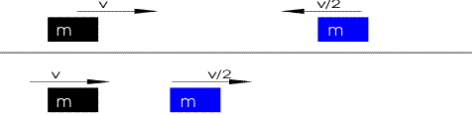
\includegraphics[scale=.6]{pic1.png}
		\newline
		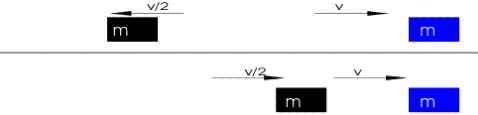
\includegraphics[scale=.6]{pic2.png}
		
	\end{figure}
	
	Profiling reveals this area of the implementation as a  computational hotspot as the problem size increases. This is due to a number of expensive operations (multiplication and square root) being called for each unique pairing of objects.\newline
	
	This can be approximated as $!n \times t$ calls for each operation where $n$ is the number of objects and $t$ is the number of time steps.  \newline
	\subsection{Verification}
	
	The following steps have been taken to verify the implementation:
	
	\begin{itemize}
		\item Check functionality at small object and time step values
		\item Print all position and velocity values into a file and manually check physics.
		\item Print all collisions and related object information into file upon occurance
	\end{itemize}
	
	As discussed briefly in the previous section, the collision physics used in the collision handling will not be valid for angled collisions. This will be corrected in future implementations by separating collision logic into head collisions and angled collisions.\newline
	
	In future revisions, object positions may be visualised with an external program to further verify correctness.
	
	%------------------------------------------------
	\newpage
	\subsection{Serial Performance}
	Results of performance scaling with problem size can be seen in table 1. \newline
	\begin{table}[H]
		\caption{Performance (run time) over number of objects}
		\centering
		\begin{tabular}{llr}
			\toprule
			\multicolumn{2}{c}{Problem size} \\
			\cmidrule(r){1-2}
			Num. Objects & Num Timesteps & Run Time (s) \\
			\midrule
			50 & 20 & $< 0.000001$ \\
			500 & 20 & $0.05$ \\
			1000 & 20 & $0.28$ \\
			5000 & 20 & $5.50$ \\
			10000 & 20 & $19.80$ \\
			500 & 100 & $0.21$ \\
			1000 & 100 & $0.70$ \\
			5000 & 100 & $13.86$ \\
			10000 & 100 & $45.00$ \\
			500 & 500 & $2.16$ \\
			1000 & 500 & $7.16$ \\
			5000 & 500 & $130$ \\
			500 & 1000 & $4.40$ \\
			500 & 5000 & $20.30$ \\
			\bottomrule
		\end{tabular}
	\end{table}	
	
	\begin{figure}[H]
		\caption{Graph of Serial Implementation Performance}
		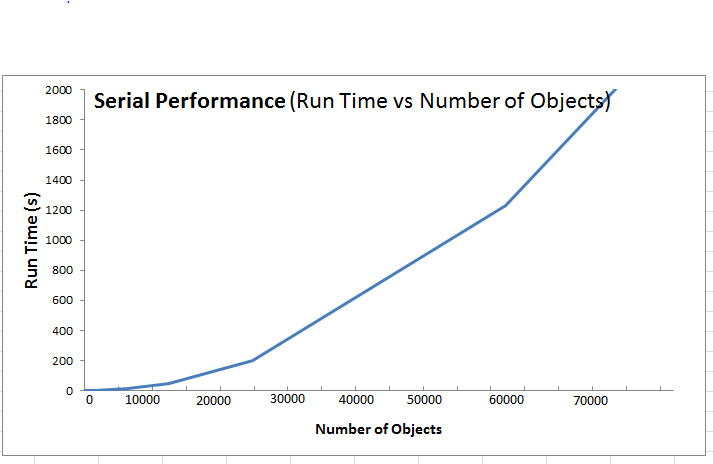
\includegraphics[scale=.6]{serial.png}
	\end{figure}
\clearpage
	%------------------------------------------------

	\section{Parallel Implementation}
	\subsection{Parallelisation and Optimisation Strategies}
	As the time portion of this problem is inherently sequential, parallelisation over the time domain is outside the scope of this project. \newline 
	Thus, the parallelisation methods used in this project can be broken down into the following (concerning the parallelisation of objects within each timestep):
	
	\begin{itemize}
		\item OpenMP parallelisation for the initialisation of all objects (including random number generation)
		\item OpenMP parallelisation for the propogation of objects forward in time
		\item MPI parallelisation to calculate collisions between every unique object pair (through domain decomposition of the list of objects)
	\end{itemize}
	
	The overall runtime speedup of the OpenMP parallelisation optimisations was expected to be minor compared to speedups through parallelisation of the collision detection and simulation routines. \newline
	This was suggested by initial profiling of the serial implementation and Big-Oh analysis of the collision detection and simulations routines (due to nested for loops with costly mathematical operations and numerous array operations within). \newline
	
	To support MPI parallisation, several adjustments needed to be implemented:
	
		\begin{itemize}
			\item Domain decomposition of the object list to facilitate parallel collision detection and simulation
			\item Maintaining a buffer of colliding object pairs which lie outside of the local domain of each thread to avoid concurrency conflicts.  \newline
			This buffer was then used to serially calculate the collisions after the local collisions had been gathered into the global object list. 
		\end{itemize}
		

	%------------------------------------------------
	
		
	%------------------------------------------------
	
	\subsection{Parallel Performance}
	Results of performance scaling with problem size can be seen in Table 1 and Figure 2. \newline
	
	\begin{table}[H]
		\caption{Average performance over problem size}
		\centering
		\begin{tabular}{llr}
			\toprule
			\multicolumn{2}{c}{Problem size} \\
			\cmidrule(r){1-2}
			Num. Objects & Parallelisation & Run Time (s) \\
			\midrule
			200 & Milestone 1 Code & $0.41s$ \\
			200 & Milestone 2 Code (serial) & $0.67s$ \\
			200 & OpenMP (2) & $0.61s$ \\
			200 & OpenMP (4) & $0.61s$ \\
			200 & OpenMP (8) & $0.61s$ \\
			200 & OpenMP (2) MPI (2) & $0.59s$ \\
			200 & OpenMP (2) MPI (4) & $0.59s$ \\
			\midrule
			2000 & Milestone 1 Code & $8.8s$ \\
			2000 & Milestone 2 Code (serial) & $8.6s$ \\
			2000 & OpenMP (2) & $6.8s$ \\
			2000 & OpenMP (4) & $6.8s$ \\
			2000 & OpenMP (8) & $6.8s$ \\
			2000 & OpenMP (2) MPI (2) & $4.3s$ \\
			2000 & OpenMP (2) MPI (4) & $2.6s$ \\
			\midrule
			5000 & Milestone 1 Code & $50s$ \\
			5000 & Milestone 2 Code (serial) & $37s$ \\
			5000 & OpenMP (2) & $37s$ \\
			5000 & OpenMP (2) MPI (2) & $24.3s$ \\
			5000 & OpenMP (2) MPI (4) & $11.1s$ \\

			\bottomrule
		\end{tabular}
	\end{table}	
	
		\begin{figure*}
			\caption{Graph of Parallel Performance (Average Run Time vs Number of Objects)}
			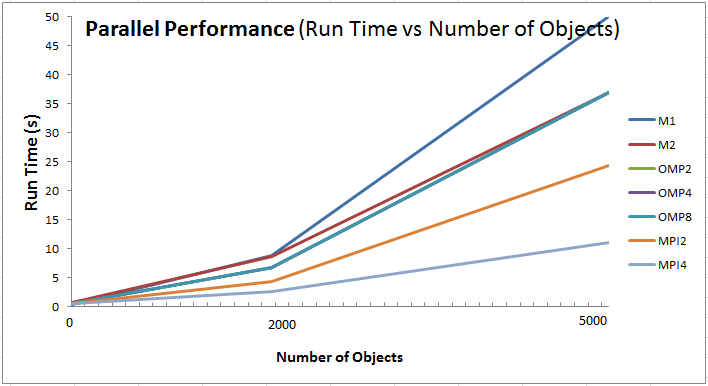
\includegraphics[scale=.9]{para.png}
		\end{figure*}
	\subsection{OpenMP Analysis}
	As suggested earlier in the report, the effectiveness of the OpenMP parallelisation in terms of overall computation speedup was minor due to comparitive cost of the collision detection and simulation. For moderately sized problems, OpenMP offered a slight improvement in run time.
	
	\subsection{MPI Analysis}
	The most effective speedups offered were by the MPI parallelisations, which resulted in significant speedups with large numbers of objects. This is a result of the performance of the implementation being bound by the collision algorithm. This analysis is further expanded on in section 4.
	
	\subsection{Verification}
	
	To verify the small scale implementation, a visualiser was built in Java which plots all of the objects within 2d space and animates over the time steps, using the output file of the C program. This visualisation is a means to verify the implementation at smaller problem sizes. \newline
	
	The visualiser is bundled with the report in both .jar file and executable form. This is also located on the repository along with the source code. \newline
	
	\begin{figure}
		\caption{Java Visualiser Demonstration}
		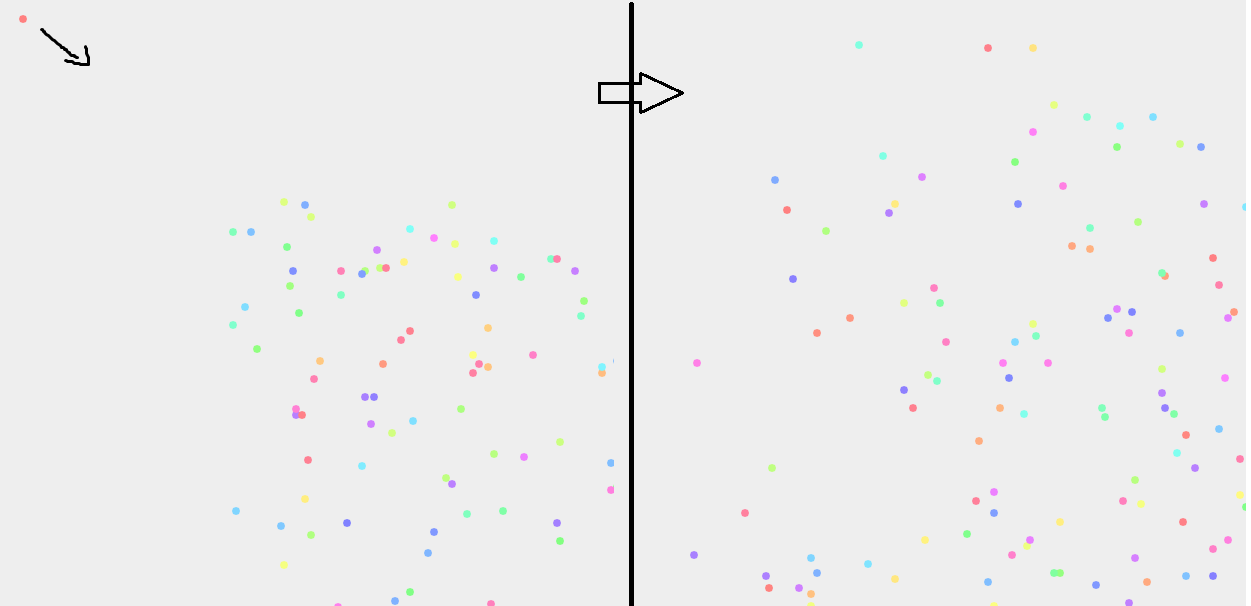
\includegraphics[scale=.25]{visEx.png}
	\end{figure}
	
	
	The bundled visualiser is able to visualise objects in the domain and range of [-200, 200] (adjustable in source code). It is worth noting that the frame rate of the visualiser suffers with large problem sizes (greater than 500 objects). \newline
	
	Further verification of the implementation can be achieved by checking individual objects in the output file. The following steps have been taken to verify the implementation: \newline
	
	\begin{itemize}
		\item Using the visualiser, check object behaviour is as expected. 
		\item Print all position and velocity values into a file and manually check physics, ensuring conservation of energy.
		\item Print all collisions and related object numbers into file upon occurance.

	\end{itemize}
	
	
	\clearpage
	
	\section{Large Scale}
	
	
	\subsection{Testing and Experimental Process}
		
		The testing process was as follows.
	
	
		Building upon the previous milestones, the following steps have been taken to verify the implementation: \newline
		
		\begin{itemize}
			\item Using the visualiser, check object behaviour is as expected. 
			\item Print all position and velocity values into a file and manually check physics, ensuring conservation of energy.
			\item Print all collisions and related object numbers into file upon occurence.
			\item Test validity of individual outputs for each thread with the above methods.
			\item Check for coherency of results between threads by printing and comparing values.
		\end{itemize}

	\subsection{Further Optimisations}
	Building toward a large scale implementation, several parts of the code were rewritten to minimise memory usage and free up memory. \newline
	
	An optimisation discovered while writing this report, was to adopt the single precision floating point data type (32 bits) as opposed to the double precision data type(64 bits). For the needs of the project, single precision had sufficient accuracy. The performance gain of this optimisation was a speed up of about 1.6x for the large scale tests.
	
	\subsection{Performance Analysis}

	Using the results of the small scale parallelisations, and after testing of large scale with various configurations, only three configurations were used for the large scale implementations. These configurations are as follows: \newline
	\begin{itemize}
		\item The serial implementation.
		\item The parallel implementation with 4 MPI ranks and 2 OpenMP threads.
		\item The parallel implementation with 8 MPI ranks.
	\end{itemize}
	
	The rationale for these configurations is as follows: \newline
	Since the algorithm used to calculate collisions between two objects is roughly O$(N^2)$, and all other algorithms used in the implementation is O$(N)$, the runtime of the implementation will be bound by the performance of the collision implementation. \newline
	Thus, the parallelisation method which will theoretically provide the most scalable speedup will be one which achieves the most parallelisation of the collision algorithm. \newline
		
	The above configurations were chosen to maximise the usage of the available resources on the cluster whilst testing the above argument. \newline
	
	\begin{figure*}
		\caption{Graph of Large Scale Performance (Average Run Time vs Number of Objects )}
		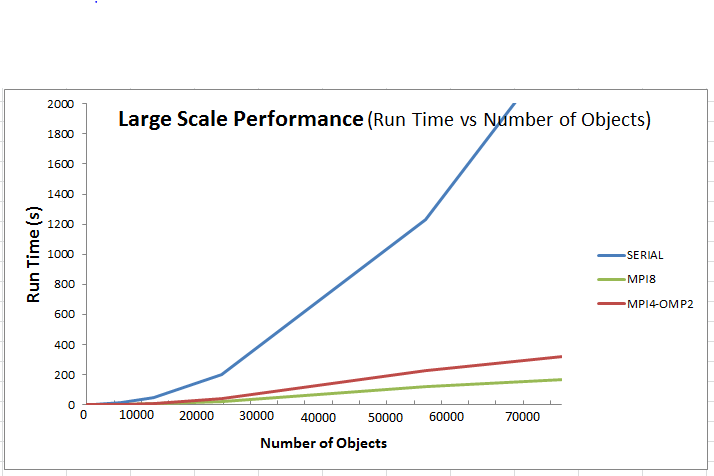
\includegraphics[scale=.8]{large.png}
		\label{large}
	\end{figure*}
 
	Regarding the bounds on the number of objects used; tests of greater than 70,000 objects caused the process on the cluster to crash. This was attributed to running out of local memory due to numerous allocations of large arrays on each MPI rank. A rewritten implementation with a focus on memory management may be able to extend this limit further. This was may be considered in future work. \newline
	
	\begin{figure*}
		\caption{Graph of Speed Up Factor (compared to Serial Implementation) vs Number of Objects}
		\label{speed}
		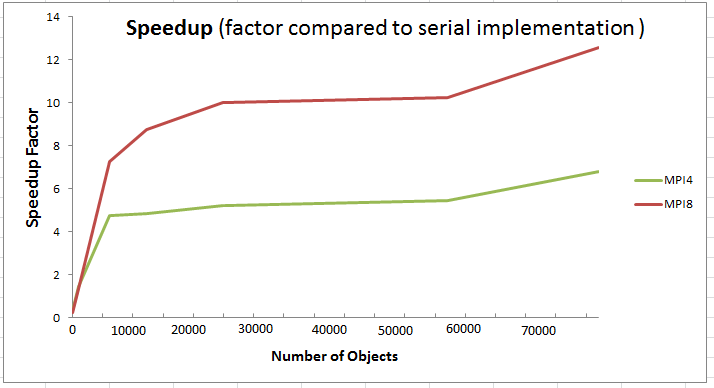
\includegraphics[scale=.8]{speed.png}
	\end{figure*}
	
	As can be seen in Figure~\ref{large}, the implementation scaled well with MPI ranks. The above theory on the optimum parallelisation configuration was supported. \newline
	
	Furthermore, for the numbers of MPI ranks used, i.e. for small numbers of nodes, the implementation appeared to have near Linear Strong Scaling. This can be seen in Figure~\ref{speed}. However, this scaling is not expected to hold as the MPI ranks further increases, with communication costs expected to quickly result in diminishing returns in performance. \newline
	
	Due to the intrinsically deterministic nature of time propagation making time parallelisation impossible as well as concurrency issues and memory usage issues plagueing the object parallelisations, there was no possible Weak Scaling. \newline
	
	In terms of asymptotic performance, the parallel implementation runs well below the serial implementation's O$(N^2)$, estimated as bounded close to (but above) O$((N/p)^2)$, where $p$ is the number of parallel MPI processes. This estimation assumes Linear Strong Scaling, which as discussed above, is not expected to hold indefinitely as $p$ increases. \newline
	
	Thus the asymptotic performance, $a$, of the parallel implementation is bounded by the following: \newline
	
	\begin{equation}
		O((N/p)^2) > a > O(N^2)
	\end{equation}
	
	\subsection{Discussion}
		
	Concerning the initially proposed scientific task (i.e. a simulation of physical collisions between 2D objects such as asteroids of pool balls), the project has demonstrated the required large scale simulation capabilities. \newline
	
	Due to the HPC focus of this project and the small room for rigorous investigation within the topic, scientific investigation relating to the topic of 2D Elastic Collisions was minimal. \newline
	
	Within the implementation itself, the most significant  problems encountered were concurrency issues and memory usage issues. Concurrency issues were resolved by doing multi-staged passes of collisions in serial after the initial parallel pass. \newline
	
	Memory usage issues were remedied primarily by tighter memory management and changing from double precision floating numbers to single precision. As discussed earlier, this contributed to a significant speedup, but also extended the memory constraints. \newline
	
	Unfortunately, memory usage issues still remained a bottleneck on the number of objects possible in parallel implementation - stemming in part from the solution to concurrency issues. The author remarks that such an issue is probably not an uncommon occurance within the parallel optimisation field. \newline
	
	Possible improvements or areas of further study may include:
		\begin{itemize}
			\item Solutions to concurrency issues.
			\item Solutions to memory usage.
			\item Decomposition of objects by location rather than arbitrary number.
			\item More efficient collision detection algorithms using reductive heuristics.
			\item Improved visualisation and verification methods.
			\item Investigation of performance in three dimensions.
		\end{itemize}
	
	
	\section{Conlusion}
	
	This report has summarised the performance and scalability of an implementation of Elastic N-Body Collisions. This problem was found to scale well with parallel MPI ranks, with the cost of communications expected to quickly become a bottleneck for larger numbers of MPI ranks. 
	
	\newpage
	
	\section{Appendix A - Collision Detection Algorithm}
	\begin{figure} [H]
		\includegraphics[scale=.8]{paraCode.png}
	\end{figure}
	
	\clearpage
	
	\section{Appendix B - Multistage Collision Algorithm}
		\begin{figure}[H]
			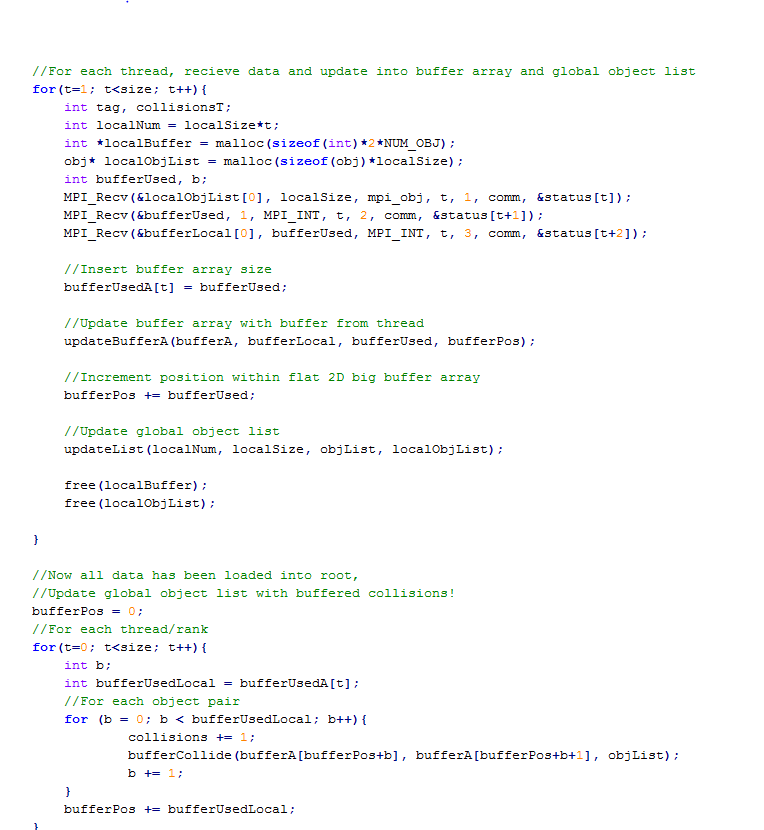
\includegraphics[scale=.7]{bufCode.png}
		\end{figure}

	%----------------------------------------------------------------------------------------
	%	REFERENCE LIST
	%----------------------------------------------------------------------------------------
	
	
	%----------------------------------------------------------------------------------------
	
\end{document}\documentclass{article}
